\documentclass{beamer}

\usepackage[english]{ babel }
\usepackage[T1]{ fontenc }
\usepackage{ graphicx }
\graphicspath{ {./pix/} }

\usetheme[block=fill]{m}

\newlength{\blackoutwidth}
\newcommand{\blackout}[1]
{%necessary comment
  \settowidth{\blackoutwidth}{#1}%necessary comment
  \rule[-0.3em]{\blackoutwidth}{1.125em}%necessary comment
}

\title{Radare2 workshop}
\author{Writing a crack for \blackout{Age of Empire} }
\date{\today}
\institute{hack.lu 2015}

\begin{document}

\maketitle

\begin{frame}{whoami}
	\begin{block}{Julien (jvoisin) Voisin}
	\begin{itemize}
		\item French
		\item Freshly graduated
		\item I don't know Windows
	\end{itemize}
	\end{block}
\end{frame}

\begin{frame}{Disclaimer}
	\begin{center}
		Piracy is \alert{bad}, m'kay.
	\end{center}
\end{frame}

\begin{frame}{What is this?}
	\begin{center}
		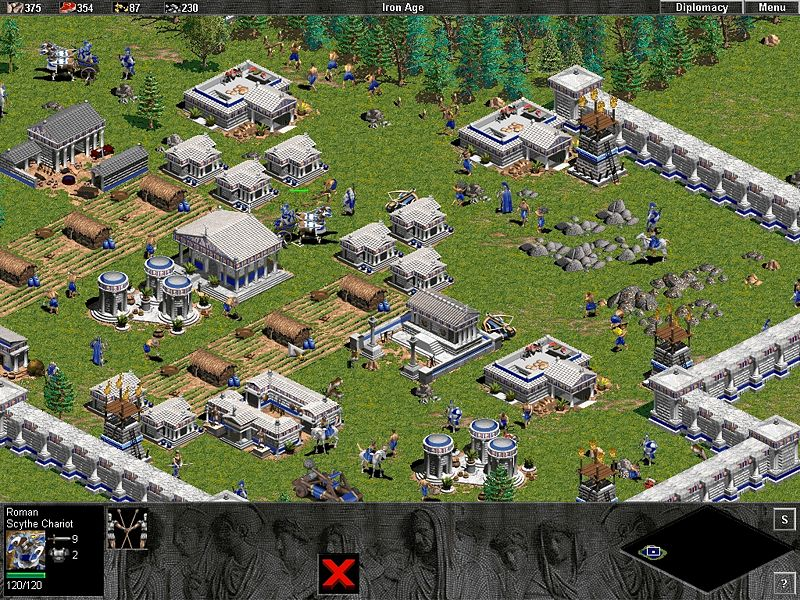
\includegraphics[width=.9\textwidth]{aoe.jpg}
	\end{center}
\end{frame}

\begin{frame}{And what is this?}
	\begin{center}
		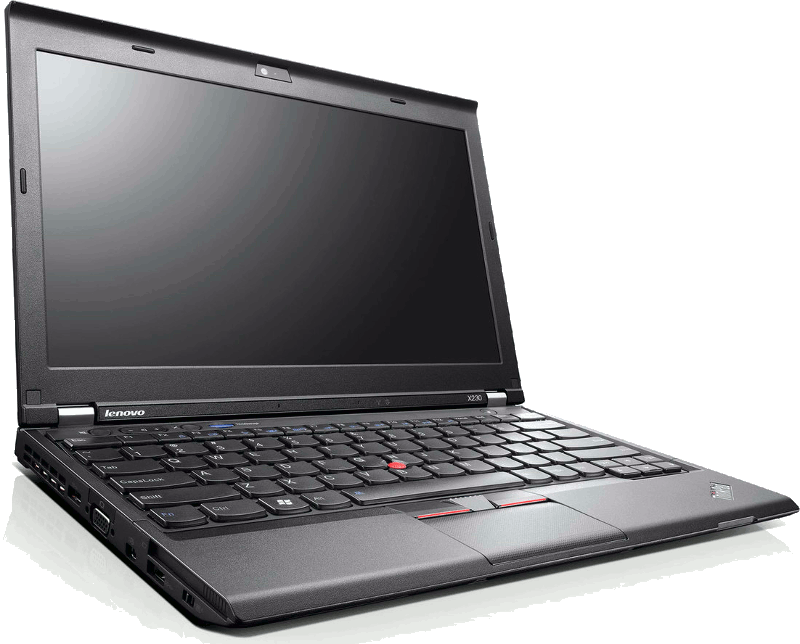
\includegraphics[width=.75\textwidth]{x230.png}
	\end{center}
\end{frame}

\begin{frame}{But I still want to play!}
	Time to write a \alert{compatibility enhancement hotfix}!
	\vskip1em
	\pause
	While knowing close to nothing about the Windows world.
\end{frame}

\begin{frame}{Finding the right function}
	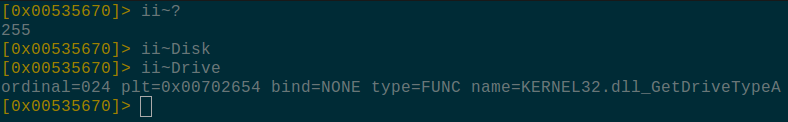
\includegraphics[width=\textwidth]{ii.png}\\
\end{frame}

\begin{frame}{Lets script some documentation fetcher for r2}
	\begin{center}
		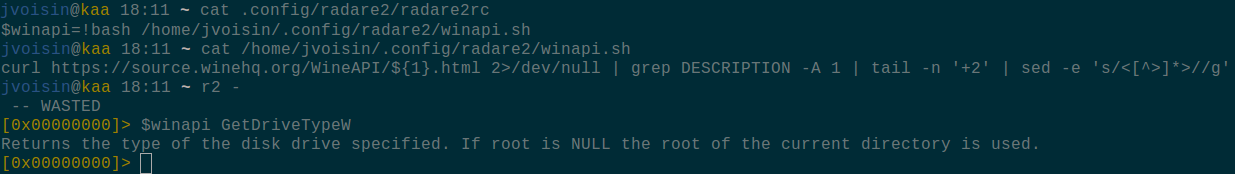
\includegraphics[width=\textwidth,height=.3\textheight]{script.png}\\
		\pause
		You've got this one in your .radare2rc in the VM
	\end{center}
\end{frame}

\begin{frame}{Find where it's called}
	\begin{block}{Your turn!}
		\begin{itemize}[<+->]
			\item Find where \alert{GetDriveTypeA} is called
			\item It's likely an \alert{a}nalysis command, about \alert{x}ref \alert{t}o something
			\item There are two locations:
				\begin{itemize}
					\item \emph{0x4d65f6}
					\item \emph{0x5352ee}
				\end{itemize}
			\item In what function do they belong?
			\item Still in \alert{a}nalysis, \alert{f}unction related, about \alert{i}nformation
			\item \emph{afi 0x4d65f6}
			\item \emph{afi 0x5352ee}
		\end{itemize}
	\end{block}
\end{frame}

\begin{frame}{Find where it's called (cont.)}
	\begin{block}{Your turn!}
		\begin{itemize}[<+->]
			\item \alert{0x4d65f6} is called from two locations:
				\begin{itemize}
					\item \emph{0x004d6550}
					\item \emph{0x004ab1aa}
				\end{itemize}
			\item Which one is the relevant one? (check with \emph{VV})
			\item \alert{0x004d6550} is the cd-check routine!
		\end{itemize}
	\end{block}
\end{frame}

\begin{frame}{Patching time}
	\begin{enumerate}
		\item Reopen the binary in \alert{write} mode with \emph{oo+}
		\item Hardcode a return value for \alert{fcn.0x004d6550}
		\item Play the game without the CD!
	\end{enumerate}
\end{frame}

\begin{frame}{My solution}
	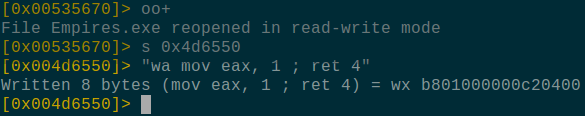
\includegraphics[width=\textwidth,height=.3\textheight]{crack.png}
\end{frame}

\section*{Conclusion}
\begin{frame}{Conclusion}
	\begin{center}
	\only<1>{
		\begin{itemize}
			\item Having no CD reader sucks,
			\item Age of Empire is cool,
			\item So is radare2.
		\end{itemize}
	}
	\only<2>{
		\Large
		Radare2 is \alert{nice}.

		You should use it.
	}
	\end{center}
\end{frame}

\begin{frame}{Resources}
	\begin{itemize}
		\item \href{https://github.com/radare/radare2}{Github repo}
		\item \href{http://rada.re}{Official website}
		\item \href{http://radare.today}{The r2 blog}
		\item \href{http://maijin.github.io/radare2book/}{The r2 book}
		\item \href{https://twitter.com/radareorg}{Twitter}
	\end{itemize}
\end{frame}

\end{document}
